\chapter{Généralités/Contexte}


\section{Caractéristiques générales des rouleaux de couche limite}
Structure cohérentes de la Couche Limite Atmosphérique (CLA), occupent la hauteur de la CLA. \\
Aussi bien au dessus de la mer que la terre. \\
Dû à des instabilités dynamiques et thermiques. \\
Apparaissent dans des condition de stratification neutre ou presque-neutre. \\
Observées dans de nombreuses situations (voir section),souvent associées à des rues de nuages. la définition ne semble pas très claire car est associé à des forces de vents et des situations très variées. mais lien entre troposphère et surface donc intéressant. 

\begin{figure}[h!]
	\centering
	
\includegraphics[width=0.75\textwidth]{Etling.png}
	\caption{Caractéristiques des rouleaux (figure modifées et infos de \cite{etlingRollVorticesPlanetary1993})}
\end{figure} 

\section{Definition de termes}
rapprot d'aspect 

\section{Situation d'observations de rouleaux}
On retrouve des rouleaux dans de nombreux contextes que je détaille ici. Les caractéristiques sont néanmoins différentes et peut être des processus différents expliquent la présence de structure turbulente organisées. 

\subsection{Couche Limite continentale}
\cite{weckwerthObservationalStudyEvolution1999}: Observation sur continent, évolution rlx, rapports de 1.1 à 4; $\zeta$ inutile pour formation (plutôt Ra ou flux de H) mais utile pour voir la fin ($\zeta < 25$). \\
Évolution convection 2D à 3D sur continent. \\
Peut être dû aussi à des hétérogénéités de surface (\cite{marongaLargeEddySimulationsSurface2012}) dans des LES idéalisées. Etude de même du cycle diurne. Corrélation rouleaux et hétérogénéités visible si moyenne assez longue. 




\subsection{Cyclones extra-tropicaux}
\begin{itemize}
\item Observation de rouleaux dans une simulation du cyclone méditerranéen Adrian en 2019 dans des simulations LES (\cite{lfarhImpactSurfaceTurbulent2024}). Présente l'importance des flux de chaleurs sensible, jet de basse couche froid sur mer Méditerranéenne chaude. Manière de tester différentes paramétrisations atm-mer. 

\item Dans simulation idéalisé de cyclone extra-tropical, rouleaux responsables du transport de quantité de mouvement vers la surface (\cite{riviereDownwardTransportMomentum2020}) à l'arrière de la tête nuageuse lorsqu'il y a du refroidissement par évaporation ou sublimation. Faible valeur du nombre de Richardson.  \\

"our interpretation is that the convective rolls are
formed by destabilization of the air masses at the precipi-
tation base via CDI [cloud-base detrainment insta-
bility], and the associated air masses continue
their descent because they met favorable conditions for
convective instability further below the precipitation base."

cf Browning et al 2015 ?

\item SAR + LES de Nicolas Maury (attente de papier)
\end{itemize}




\hl{Quelle instabailité est derrière ??}
peut être DI = vent froid sur mer chaude  => instabilité thermique ? \\l
low level jet => instabilité dynamique x thermique ? 
plutôt cellules ? 

\subsection{Hurricanes}
\begin{itemize}
	\item  étude théorique \cite{foster2005}
	\item simulation réel de Ivan par Zhu 208
	\item cas idéalisé de CL de hurricane (\cite{nakanishiLargeEddySimulationRoll2012})
\end{itemize}



\subsection{Cold Air Outbreak}
What is CAO ? "Maritime CAOs are atmospheric phenomena entailing equatorward excursions of cold polar air masses over the relatively warm adjacent open ocea" , difference in tempeature at the atmosphere-ocean interface. 
\begin{itemize}
	\item simulation cas idéalisé (\cite{chlondThreedimensionalSimulationCloud1992})
	\item (\cite{brummerRollCellConvection1999}) observation de rouleaux $2.6 < \lambda /H < 6.5 $. près bord de glace: rouleaux qui grossissent puis des cellules. Observations avec 13 vols. Comparaison entre les rouleaux et cellules sur les vitesses, condensation, températures, flux... 
	indice de - d'importance de l'humidité dans les rouleaux que dans les cellules car 
	\begin{figure}[h!]
		\centering
		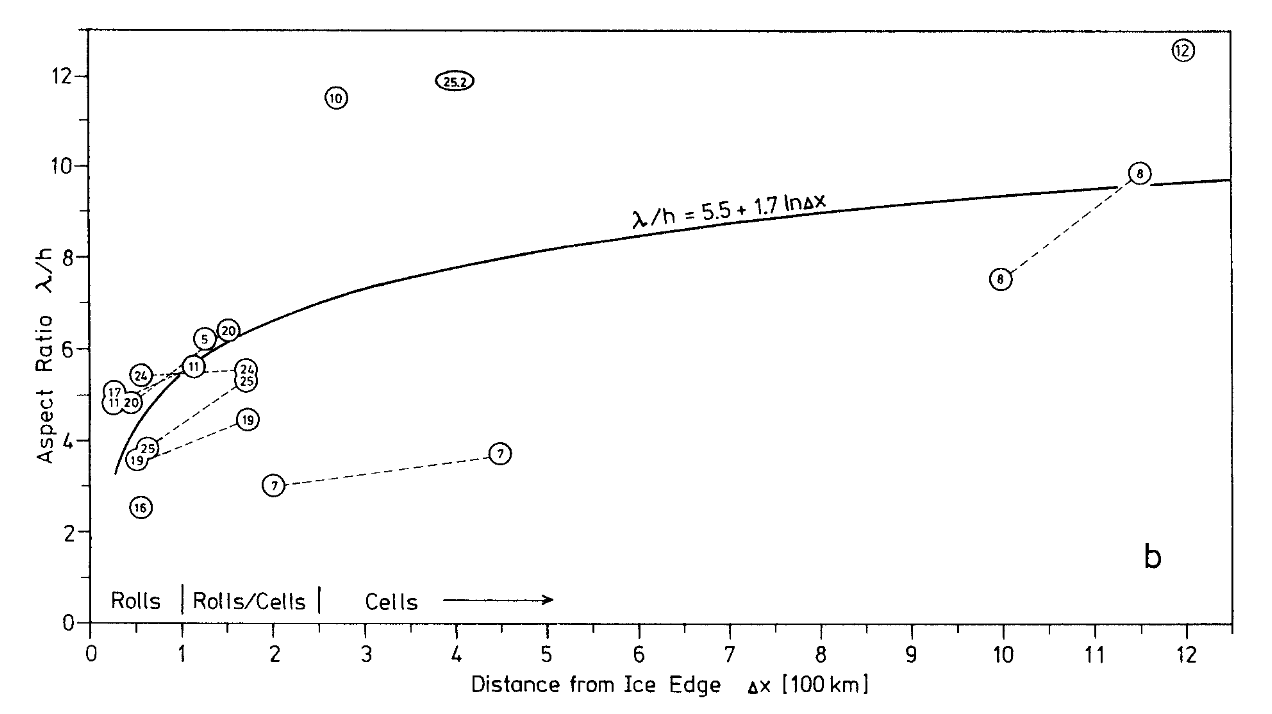
\includegraphics[width=0.7\linewidth]{FIGURES/Brummer_graph1}
		\caption{}
		\label{fig:brummergraph1}
	\end{figure}
	
	\item Simulation idéalisée (\cite{gryschkaImpactForcedRoll2014}), même paramètre de stabilité que brummer , importance d'hétérogénéité de surface dans la formation des rouleaux dans la LES. Impact des structures organisées sur le transport de quantité de mouvement négligeables comparées au mélange turbulent. 
	question cmt rolls sur interaction ocean mixed level and atm boudary layer ?
	muller et al 2013 réponse de l'océan était faible mais puet etre sous estimé par manque résolution de phénomène de petite échelle 
\end{itemize}


\subsection{Monsoon}

fractional area of of rising motion $\sigma$ ??


\subsection{Hétérogéniité de flux de surface}


feedback avec ombres des nuages


\begin{table}[h!]
	\begin{tabular}{c||c ||c|c|c|c}
		ref                                            & evt       & U & $\zeta$     & $\lambda / z_i$ &  Mesure\\
		\hline \hline			
		\cite{brummerRollCellConvection1999}           & CAO       & 15  &           & 2.6 - 6.5       & avion\\
		\cite{weckwerthObservationalStudyEvolution1999}& Continent & mid &$<25$      & 1.1 to 4        & sol, Radar\\
		\cite{foster2005}                              & Hurricane & 40  &$\approx 0$& 2.4             & SAR + ground
	\end{tabular}
\end{table}



\section{Instabilités}


\section{Définition}
Qu'est ce que c'est ??

\section{Instabilités dans d’atmosphère liées aux échelles et processus}

\section{Les instabilités de la couche limite}
\subsection{Instabilité thermique}
\textbf{instabilité thermique}: Cause principale de l'apparition de tourbillon en rouleaux. Convection de Rayleigh Bénard. Explique pk rolls surtout observés au dessus de la mer pendant CAO et au dessus de la terre durant la journée.\\

Mais aussi une importance de l'évaporation et sublimation (evaportative cooling) (\cite{riviereDownwardTransportMomentum2020}). Peut etre aussi du au refroidissiement radiatif des stratus mais attention resolution verticale très fine necessaire (Lilly, de Lozar \& Mellado (2015) Mellado (2017)
\subsection{Instabilité dynamique}
\textbf{instabilité d'inflection} : lié au cisaillement de vent dans une couche d'Ekmann. Le profil de vorticité admet un max qui coincide avec le max de vitesse v qui est un point d'inflection. $\lambda/H = 3$. Condition : point d'inflection $<0.6 z_i$. instabilité très faible dans une CLA turbulente. 

\subsection{Instabilité parallèle}
\textbf{instabilité parallèles} Seulement dans écoulement rotatif. Rouleaux plus étendu $\lambda/H = 6$

Dûs à des instabilités de cisaillement et thermiques. A distinguer des cellules. Les différentes

\section{Différents types d'instabilités: } 




\subsection{Paramètre $\zeta$ ou nombre de Richardson}
\paragraph{Nombre de Richardson $Ri$}: ratio flottabilité sur cisaillement. 
\begin{equation}
Ri = \frac{\frac{g}{T_v}\frac{\partial \theta_v}{\partial z}}{\left(\frac{\partial u}{\partial z}\right)^2 + \left(\frac{\partial v}{\partial z}\right)^2 }
\end{equation}
Lorsque Ri est positif : mélange turbulent à l'inverse quand négatif c'est convectif.


\paragraph{Paramètre de stabilité statique $N_v^2$}: Info sur instabilité convective. 
N = Brunt Väisälä frequency 
\begin{equation}
	N_v^2 = \frac{g}{\theta_v} \frac{\partial \theta_v}{\partial z}
\end{equation}
si $<0$ instable convectivement, 

\paragraph{Longueur de Monin-Obukhov $L$}: hauteur à partir de laquelle la turbulence est créée plus par flottabilité que par cisaillement de vent. 

\paragraph{Paramètre $\zeta$} Définit avec hauteur de couche limite $z_i$ et longueur de Moonin-Obukhov $L$. \hl{trouver lien avec Ri}
Paramètre de stabilité  
$$\zeta = -\frac{z_i}{L}$$
 : différencie les types de convection / influence flottabilité vs cisaillement.\\ 
où $L$, la longueur de Monin et Obukhov = - la distance où la turbulence produite par la flottabilité est supérieure à celle du cisaillement. \\
Pour $\zeta >> 1$ on est dans une situation purement convective. Des rouleaux sont oservés pour $\zeta \approx 0.5 < 1$ (\cite{lfarhImpactSurfaceTurbulent2024}) donc dans un BL neutre. \\
Les rouleaux sont attendus entre $6<\zeta<15$ (\cite{etlingRollVorticesPlanetary1993}), interaction entre convection et cisaillement. Mais aussi pour $\zeta \approx 2$ dans le cas d'une instabilité d'inflection. \\
C'est aussi souvent le cas pour $\zeta < 10$ ('free rolls') mais aussi pour $>20$ forced rolls
(\cite{gryschkaImpactForcedRoll2014}) \\



\begin{figure}[h!]
  \begin{center}
    
\includegraphics[width=0.7\textwidth]{Young2002.png}
  \end{center}
  \caption{Figure de \cite{youngSupplementRollsStreets2002}}\label{fig:}
\end{figure}


\section{Distinction type de rouleaux }
\cite{gryschkaImpactForcedRoll2014} propose de distinguer
\begin{itemize}
	\item "Free rolls": dû à l'organisation de l'écoulement $\propto \zeta$
	\item "Forced rolls": dûs au hétéorgénéité de surface $\propto$ hétéorgénéités 
\end{itemize}


\section{Problématiques/Questions de recherche}
Transport de vent forts vers la surface ex Sting jet dans les cyclones extra-tropicaux. 
Transport d'humidité et échange avec l'océan FLux chaleur sensible et latente ex gryschka dans les CAO peut aider la cyclogénèet ou dvp d'uhrrican ex Forster. 
Pas résolu pour grande maille, mal parapétrisé. influence sur les transports
Interessant d'avoir influence nuage/convection



\paragraph{Distinguer un rouleau}
paramètre d'autocroorélation spatiale R, puis facteur d'applatsissement f pour avoir l'allongement de la structure (\cite{lfarhImpactSurfaceTurbulent2024}).

\paragraph{Paramètre de stratification}

